\subsection[Realidade Aumentada]{Realidade Aumentada}
\begin{frame}
\frametitle{Realidade Aumentada}

A realidade aumentada � uma t�cnica de vis�o
computacional em que valendo-se de artefatos do mundo real, tem por objetivo
causar sensa��o de imers�o do usu�rio em um ambiente aumentado por artefatos virtuais, ao contr�rio de ambientes puramente virtuais 
como � comum em aplica��es de realidade virtual
\end{frame}

\begin{frame}
\frametitle{Realidade Aumentada Aplicada}


\begin{figure}[H]
\centering
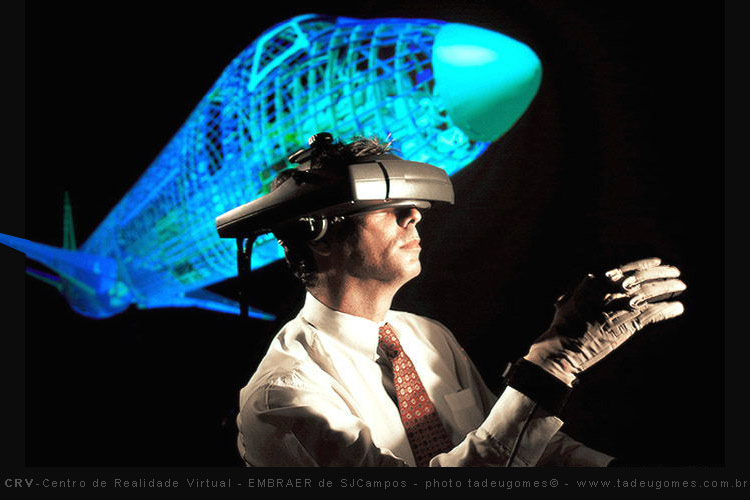
\includegraphics[scale=0.2]{images/realidade-virtual}
\caption{Ambiente Imersivo. Fonte CRV EMBRAER}
\label{fig:rv}
\end{figure}


\end{frame}


\begin{frame}
\frametitle{Realidade Aumentada Aplicada}


\begin{figure}[H]
\centering
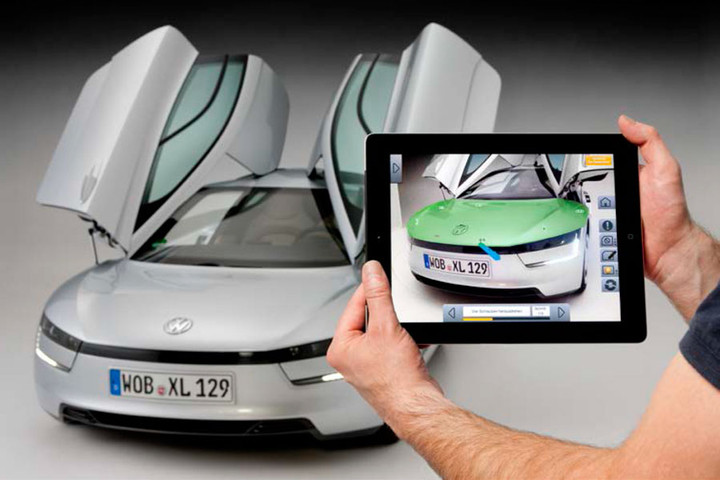
\includegraphics[scale=0.2]{images/ar}
\caption{Aplica��o de Realidade Aumentada no meio automobil�stico
Fonte www.metaio.com.br}
\label{fig:reconhecimento}
\end{figure}


\end{frame}




\begin{frame}

\frametitle{Processo de Realidade Aumentada}

\begin{figure}[H]
\centering
\begin{tikzpicture}[scale=0.9 ,transform shape]

  \node[draw,rectangle] (a) {Captura};
  \node[draw,rectangle,below of=a] (b) {Prepara��o};
  \node[draw,rectangle,below of=b] (c) {Detec��o};
  \node[draw,rectangle,below of=c] (d) {Reconhecimento};
  \node[draw,rectangle,below of=d] (e) {Rastreio};
  \node[draw,rectangle,below of=e] (f) {Apresenta��o};

  % 1st pass: draw arrows
  \draw[vecArrow] (a) to (b);
  \draw[vecArrow] (b) to (c);
  \draw[vecArrow] (c) to (d);
  \draw[vecArrow] (d) to (e);
  \draw[vecArrow] (e) to (f);
    
    
  % 2nd pass: copy all from 1st pass, and replace vecArrow with innerWhite
  \draw[innerWhite] (a) to (b);
  \draw[innerWhite] (b) to (c);
  \draw[innerWhite] (c) to (d);
  \draw[innerWhite] (d) to (e);
  \draw[innerWhite] (e) to (f);

  % Note: If you have no branches, the 2nd pass is not needed

\end{tikzpicture}
  \caption{Processo Can�nico de Realidade Aumentada}
  \label{diagram:pipelinera}

\end{figure}


\end{frame}